\documentclass[]{report}   % list options between brackets

\usepackage{aliascnt} 
\usepackage{hyperref} 
\usepackage{MnSymbol}
\usepackage[pdftex]{graphicx}

% type user-defined commands here

\begin{document}

\title{Objeck Programmng Language}   % type title between braces
\author{Randy Hollines}         % type author(s) between braces
\date{\today}    % type date between braces
\maketitle

\begin{abstract}
Objeck is an object-oriented computer language with functional
features. The language has ties with Java, Scheme and UML. In this 
language all data types, except for higher-order functions, are treated as objects.
\end{abstract}

\label{Introduction}
\chapter{Introduction}
The Objeck program language is an object-oriented computer language
with functional features.  The language was designed to be an easy to
use general purpose programming system.  The Objeck language allows
programmers to quickly create solutions by leveraging existing class
libraries and APIs.  The syntax for the language was designed with
symmetry in mind and enforces the notion that there should one
intuitive way to do things. Features include:
\begin{itemize}
\item Support for object-oriented programming (all data types are
  treated as objects)
\item Functional support (higher-order functions)
\item Unicode support with external UTF-8 encoding/decoding
\item Cross platform (support for OS X, Linux and Windows)
\item Concurrent runtime JIT support
\item Multi-threaded memory garbage collector
\item Local optimizations including method inlining
\item Support for static libraries
\item Command line debugger
\end{itemize}

\chapter{Getting Started}

The Objeck distribution consists of a compiler, virtual machine,
debugger and library inspection tool.  The compiler executable is
named \texttt{obc}, while the runtime virtual machine (VM) executable
is named \texttt{obr}.  Here is the world famous ``Hello World"
program written in the Objeck language:

\begin{verbatim}
class Hello {
  function : Main(args : String[]) ~ Nil {
    "Hello World!"->PrintLine();
  }
}
\end{verbatim}

\section{Compiling Source}
The example below compiles the source program \texttt{hello.obs} into
the target binary file \texttt{hello.obe}.  The two output file types
that the compiler supports are executables and shared libraries.
Shared libraries are binary files that contain all of the metadata
needed by the compiler to relink them into executables.  Both
executables and shared libraries contain enough metadata to support
runtime introspection.  As a naming convention, executables must end
in \texttt{*.obe} while shared libraries must end in \texttt{*.obl}.

Below is an example of compiling the ``Hello World" program:
\begin{verbatim}
obc -src tests\hello.obs -dest hello.obe
\end{verbatim}

Here's a more advanced example of linking in two required class
libraries to an executable.
\begin{verbatim}
obc -src examples\xml_parser.obs -lib collect.obl,xml.obl -dest a.obe
\end{verbatim}

Additional compiler options are:
\begin{table}
  \begin{tabular}{| l | l |}
    \hline
    \emph{Option} & \emph{Description} \\ \hline \hline
    \texttt{-src} & path to source files, delimited by the `\texttt{,}' character \\ \hline
    \texttt{-lib} & path to library files, delimited by the `\texttt{,}'
    character\\ \hline
    \texttt{-tar} & target output \texttt{exe} for executable and \texttt{lib} for library; default is  \texttt{exe} \\ \hline
    \texttt{-opt} & optimization level \texttt{s0}--\texttt{s3} with \texttt{s3} being the most aggressive; default is \texttt{s0} \\ \hline
    \texttt{-dest} & output file name \\ \hline
    \texttt{-alt} & compile code that is written using a C-like syntax \\ \hline
    \texttt{-debug} & if set, produces debug out for use by the interactive debugger (see below) \\ \hline
  \end{tabular}
\end{table}

\section{Executing}
The command-line example below executes the \texttt{hello.obe}
executable. Note, for executables all required libraries are
statically linked in the target output file.  When compiling shared
libraries, other shared libraries are \underline{not} linked into the
target output library file.

\begin{verbatim}
obr hello.obe
\end{verbatim}

\chapter{The Basics}
Now lets introduce the core features of the Objeck programming
language.  \vspace{\baselineskip}

Let's first start with a list of keywords that exist in language.
These words are reserved for the language and may not be used as
identifiers.

\begin{table}
  \begin{tabular}{ | c | c | c | c | c | }
    \hline
    \multicolumn{5}{|c|}{\emph{Keywords}} \\ \hline \hline
    --- & @parent & --- & @self & --- \\ \hline
    and & As & Bool & break & bundle \\ \hline
    Byte & Char & class & critical & do \\ \hline
    each & else & enum & false & Float \\ \hline
    for & from & function & if & Int \\ \hline
    interface & label & leaving & method & native \\ \hline
    New & or & other & Parent & private \\ \hline
    return & select & --- & static & true \\ \hline
    TypeOf & use & virtual & while & xor \\ \hline
  \end{tabular}
\end{table}

In Objeck, all data types (excluding higher-order functions) are
treated as objects. Basic objects provide supports for boolean,
character, byte, integer and decimal types.  These basic objects can
be used to create more complex user defined objects.  The listing
below defines the basic objects that are supported in the language:

\begin{table}
  \begin{tabular}{| l | l |}
    \hline
    \emph{Type} & \emph{Description} \\ \hline \hline
    \texttt{Char} & 2 or 4 byte character \\ \hline
    \texttt{Char[]} &  character array \\ \hline
    \texttt{Bool} &  boolean value \\ \hline
    \texttt{Bool[]} &  boolean array \\ \hline
    \texttt{Byte} &  1--byte integer \\ \hline
    \texttt{Byte[]} &  byte array \\ \hline
    \texttt{Int} &  4--byte integer \\ \hline
    \texttt{Int[]} &  integer array \\ \hline
    \texttt{Float} &  8--byte decimal \\ \hline
    \texttt{Float[]} &  decimal array \\ \hline
    \texttt{Function} &  4--byte integer pair \\ \hline
  \end{tabular}
\end{table}

As mentioned above, basic types are objects and have associated
methods for each basic class type.  For example:

\begin{verbatim}
13->Min(3)->PrintLine();
3.89->Sin()->PrintLine();
-22->Abs()->PrintLine();
Float->Pi()->PrintLine();
\end{verbatim}

\section{Alternative Syntax}
The syntax of the language is based on UML which has ties with Pascal.  Given 
the popularity of the C-style languages Objeck supports an alternative C-like 
syntax.  In this mode, operators can be defined using a C-style syntax and 
statements such as \texttt{if}, \texttt{while}, etc., do not have to end with 
a semicolon.

In order to use this feature code must be compiled using the \texttt{-alt} 
compiler option.

\begin{verbatim}
a = 13;
if(13 != a) {
  for(i = 0; i < a; i+=1) {
    i->PrintLine();
  }
}
\end{verbatim}

\section{Variable Declarations}
Variables can be declared for all of the basic types (described
above), user defined objects and high-order functions. Variables can
be declared anywhere in a program and are bound to traditional block
scoping rules.  Variable assignments can be made during a declaration
or at any other point in a program. Variables may be declared as
local, instance or class level scope.  Class level variables are
declared using the \texttt{static} keyword. A class that is derived
from another class may access it's parents variables if the parent
class is declared in one of the source programs.  \textit{If a class
  is derived from a class declared in a shared library then that class
  cannot access it's parents variables, unless an accessor method is
  provided.}  Local variables can be declared without specifying their
data type, such variables are bound to the type defined by their first
right-hand side assignment. Three different declaration styles are
shown below:

\begin{verbatim}
a : Int;
b : Int := 13;
c := 7; # implicit type deceleration 
\end{verbatim}

Types that are not initialized at declaration time are initialized
with the following default values:

\begin{table}
  \begin{tabular}{| l | c |}
    \hline
    \emph{Type} & \emph{Initialization} \\ \hline \hline
    \texttt{Char} & `\textbackslash0' \\ \hline
    \texttt{Byte} & 0 \\ \hline
    \texttt{Int} & 0 \\ \hline
    \texttt{Float} & 0.0 \\ \hline
    Array & \texttt{Nil} \\ \hline
    Object & \texttt{Nil} \\ \hline
    Function & \texttt{Nil} \\ \hline
  \end{tabular}
\end{table}

\section{Expressions}
The Objeck language supports various types of expressions.  Some of
these expressions include mathematical, logical, array and method
calls.  The preceding sections describes some of the expressions that
are supported in Objeck.

\subsection{Mathematical and Logical Expressions}
The following code example demonstrates two ways to printing the
number \texttt{42}.  The first way invokes the \texttt{PrintLine()}
method for the literal \texttt{42}.  The second prints the product of
a variable and a literal.

\begin{verbatim}
class Test {
  function : Main() ~ Nil {
    42->PrintLine();
    eiht := 8;
    (eiht * 7)->PrintLine();
  }
}
\end{verbatim}

The following mathematical operators are supported in the Objeck
language for integers and decimal types:
\begin{itemize}
\item addition (\texttt{+})
\item subtraction (\texttt{-})
\item multiplication (\texttt{*})
\item division (\texttt{/})
\item modulus -- (\texttt{\%} - for integer values only)
\item shift left -- (\texttt{<<} - for integer values only)
\item shift right -- (\texttt{>>} - for integer values only)
\end{itemize}

In addition the following assignment operators are supported:
\begin{itemize}
\item addition-equals or string concatenation (\texttt{+=})
\item subtraction-equals (\texttt{-=})
\item multiplication-equals (\texttt{*=})
\item division-equals (\texttt{/=})
\end{itemize}

The following bitwise operators are also supported for integer types:
\begin{itemize}
\item and (\texttt{and})
\item or (\texttt{or})
\item xor (\texttt{xor})
\end{itemize}

The [\texttt{*}, \texttt{/}, \texttt{\%}] operators have a higher
precedence than the [\texttt{+}, \texttt{-}] operators and are
naturally enforced by the language. Operators of the same precedence
are evaluated from left-to-right.  Logical operations are of lower
precedence than mathematical operations. All logical operators are of
the same precedence and order is determined via left--to--right
evaluation.  The [\texttt{\&}, \texttt{|}] logical operators use
short-circuit logic; meaning that some expressions may not be executed
if evaluation criteria is not satisfied.

The following logical operators are supported in the Objeck language:
\begin{itemize}
\item unary not (\texttt{!})
\item and (\texttt{\&})
\item or (\texttt{|})
\item equal (\texttt{=})
\item not--equal (\texttt{<>})
\item less--than (\texttt{<})
\item greater--than (\texttt{>})
\item less--than--equal (\texttt{<=})
\item greater--than--equal (\texttt{>=})
\end{itemize}

\subsection{Arrays}
Objeck supports single and multi-dimensional arrays.  Arrays are
allocated dynamically from the system heap.  The memory that is
allocated for arrays is managed automatically by the garbage
collector.  All of the basic types described above (as well as user
defined types) can be allocated as arrays.  The code example below
shows how a two-dimensional array of type \texttt{Int} is allocated
and dereferenced.

\begin{verbatim}
array := Int->New[2,3];
array[0,2] := 13;
array[1,0] := 7;
\end{verbatim}

The size of an array can be obtained by calling the array's
\texttt{Size()} method.  The \texttt{Size()} method will return the
number of elements in a given array.  For a multi-dimensional array
the \texttt{Size()} method returns an array of sizes for each
dimension. 

The following example allocates an array of \texttt{Widget} objects.
An object must implment it's \texttt{New} method if it's going to be
instnatanced.

\begin{verbatim}
class Widget {
  New() {
  }
}

class MakeWidgets {
  function : Main(args : String[]) ~ Nil {
    widgets := Widget->New[1000];
    each(i : widgets) {
      widgets[i] := Widget->New();
    };
  }
}
\end{verbatim}

\subsection{Characters and Strings}
All characters are Unicode encoded and stored internally in the format of the host operating system.  On Windows characters are stored internally as UTF-16 (2-byte) values.  On Linux and OS X characters are stored internally as UTF-32 (4-byte) values.  On all platforms characters are read and written in UTF-8, which is ASCII compatible.  

Methods are provided to convert Unicode character arrays to UTF-8 bytes and vice versa.  Character array literals are allocated as \texttt{String} objects.  The \texttt{String} class provides support for advanced string operations (see below).

\begin{verbatim}
string := "Hello World!";
string->Size()->PrintLine();
strings := ["Hello","World!"];
sizes := strings->Size();
sizes[0]->PrintLine();
sizes[1]->PrintLine();
\end{verbatim}

\subsection{Conditional Expressions}
There's also support for ternary conditional expressions.  For example
the following statement prints the value \texttt{false} after two
logical comparisons.

\begin{verbatim}
a := 7;
b := 13;
(((a < 13) ? 10 : 20) >  15)->PrintLine();
\end{verbatim}

\section{Statements}
Besides providing support for declaration statements the language has
support for conditional and control statements.  As with other
languages, control statements can be nested in order to provide finer
grain logical control. General control statements include \texttt{if}
and \texttt{select} statements. Basic looping statements include
\texttt{while}, \texttt{do/while}, \texttt{for} and \texttt{each}
loops.  Note, all statements end with the `\texttt{;}' character.

\subsection{If Statement}

An \texttt{if} statement is a control statement that executes an
associated block of code if it evaluates to \texttt{true}.  If the
evaluation statement does not evaluate to \texttt{true} than an
\texttt{else if} statement may be evaluated (if it exists), otherwise
an \texttt{else} statement will be executed (if it exists).  The
example below demonstrates an \texttt{if} statement.

\begin{verbatim}
value := Console->ReadLine()->ToInt();
if(value <> 3) {
  "Not equal to 3"->PrintLine();
}
else if(value < 13) {
  "Less than 13"->PrintLine();
}
else {
  "Some other number"->PrintLine();
};
\end{verbatim}

\subsection{Select Statement}

A \texttt{select} statement maps a value to 1 or more labels.  Labels
are associated to statement blocks.  A label may either be a literal
or an \texttt{enum} value.  Multiple labels can be mapped to the same
statement block.  Below is an example of a \texttt{select} statement.

\begin{verbatim}
select(v) {
   label Color->Red: {
      "Red"->PrintLine();
   }

   label 9:
   label 19: {
      v->PrintLine();
   }

   label 27: {
      (3 * 9)->PrintLine();
   }
  
   other: {
     "some rather another"->PrintLine();
   }
};
\end{verbatim}

\subsection{While Statement}

A \texttt{while} statement is a control statement that will continue
to execute it's main body as long as it's conditional expression
evaluates to \texttt{true}.  When its conditional expression evaluates
to \texttt{false} than the loop body will cease to execute.

\begin{verbatim}
i := 10;
while(i > 0) {
   i->PrintLine();
   i -= 1;
}
\end{verbatim}

\subsection{Do/While Statement}

A \texttt{do/while} statement is a control statement that will execute
it's main body at least once and continue to execute it's main body as
long as its conditional expression evaluates to \texttt{true}.  When
it's conditional expression evaluates to \texttt{false} than the loop
body will cease to execute.

\begin{verbatim}
i := 10;
do { 
   i->PrintLine();
   i -= 1;
} 
while(i > 0);
\end{verbatim}

\subsection{For Statements}

The \texttt{for} statement is another common looping construct.  The
\texttt{for} loop consists of a pre-condition statement followed by an
evaluation expression and an update statement.

\begin{verbatim}
location := "East Bay"->ToCharArray();
for(i := 0; i < location->Size(); i += 1;) {
  location[i]->PrintLine();
}
\end{verbatim}

\subsection{Each Statements}

The \texttt{each} statement is a specialized version of a \texttt{for}
statement.  The \texttt{each} loop consists of a counter variable and
a data structure that has a \texttt{Size} method, such as arrays and
\texttt{Vector} classes.  The statement iterates thru all elements in
the data structure.

\begin{verbatim}
values := Int->New[3];
values[0] := 5;
values[1] := 1;
values[2] := 0;

each(i : values) {
  values[i]->PrintLine();
};
\end{verbatim}

\chapter{User Defined Types}

\section{Enums}
Enums are user defined enumerated types.  The main use of an
\texttt{enum} is to group a class of countable values, for example
colors, into a distinct category.  Once \texttt{enum} values have been
defined they may not be assigned or associated to a other
\texttt{enum} groups or integer classes.  The valid operations for
enums are as follows:

\begin{itemize}
\item assignment (\texttt{:=})
\item equal (\texttt{=})
\item not--equal (\texttt{<>})
\end{itemize}

In addition, enum values may be used in \texttt{select} statements as
conditional tests or labels. Enums may be nested in classes as well.

\begin{verbatim}
enum Color {
  Red,
  Black,
  Green
}

class Token {
  @type : Token->Type;

  New() {
     @type := Token->Type->ARRAY;
  }

  method : public : GetType() ~ Token->Type {
     return @type;
  }

  enum Type := -100 {
    NUMBER,
    STRING,
    ARRAY,
    STRUCT
  }
}
\end{verbatim}

\section{Classes}
Classes are user defined types that allow programmers to create
specialized data types.  Classes are made up of attributes (data) and
operations (methods).  Classes are used to encapsulate programming
logic and localize information.  Operations that are associated to a
class may either be at the class level or instance level.  Class
instances are created by calling an object's \texttt{New()} function.
Note, an object instance can only be created if one or more
\texttt{New()} functions have been defined.

\subsection{Class Inheritance}
Classes may be derived from other classes using the \texttt{from}
keyword.  Class inheritance allows classes to share common
functionality.  The Objeck language supports single class inheritance,
meaning that a derived class may only have one parent.  The language
also supports virtual classes, which assures that derived classes have
been defined for all required operations declared in the base class.
Virtual classes also allow the programmer to define non-virtual
methods that contain program behavior.  Virtual classes are
dynamically associated with implementation classes at runtime.
\begin{verbatim}
class Foo {
  @lhs : Int;

  New(lhs : Int) {
    @lhs := lhs;
  }

  method : native : AddTwo(rhs : Int) ~ Int {
    return 2 + rhs;
  }

  method : virtual : AddThree(int rhs) ~ Int;

  method : GetLhs() ~ Int {
    return lhs;
  }
}

class Bar from Foo {
  New(value : Int) {
    Parent(value);
  }

  method : native : AddThree(rhs : Int) ~ Int {
    return 3 + rhs;
  }

  function : Main() ~ Nil {
    bar : b := Bar->New(31);
    b->AddThree(9)->PrintLine();
  }
}
\end{verbatim}

\subsection{Class Casting and Identification}
An object that is inherited from another object may be either upcasted
or downcasted.  Object casting can be performed using the
\texttt{As()} operator.  Upcasting requires a runtime check, while
down casting does not. If cross casting is detected then a compile
time error will be generated.

\begin{verbatim}
values := Vector->New();
values->AddBack(IntHolder->New(2));
values->AddBack(IntHolder->New(4));
values->AddBack(IntHolder->New(8));

total := 0;
each(i : values) {
  total += values->Get(i)->As(IntHolder)->Get();
};
total->PrintLine();
\end{verbatim}

To determine if an object instance is of a certain class type (object
or interface) it's \texttt{TypeOf} method can be invoked.  This method
will return \texttt{true} if the instance is of the same or a derived
type, \texttt{false} otherwise.  This method can be used to check a
class instance type before casting it.

\begin{verbatim}
s := "FooBar";
t := s->TypeOf(String);
t->PrintLine();
\end{verbatim}

The class that a given object instance belongs to can found by calling
its \texttt{GetClassID} method.  This method returns an enum that is
associated with that instance's class type.  This method is generally
used to determine if two object instances are of the same or different
classes.

\subsection{Methods and Functions}
The Objeck language supports both methods and functions.  Functions
are public static procedures that may be executed by any class.
Methods are operations that may be performed on an object instance.
Methods have \texttt{public} and \texttt{private} qualifiers.  Methods
that are \texttt{private} may only be called from within the same
class, while \texttt{public} methods may be called from other classes.
Note, methods are \texttt{private} by default. The Objeck language
supports polymorphic methods and functions, meaning that there can be
multiple methods with the same name within the same class as long as
their declaration arguments vary.

Method and function parameters may also be assigned default values.  For example:
\begin{verbatim}
function : Duplicate(str : String, max : Int := str->Size()) 
         ~ String { ... }
\end{verbatim}

Methods and functions can either be executed in an interpreted or JIT
compiled mode. Interpreted execution mimics microprocessor functions
in a platform independent manner. JIT execution takes the compiled
stack code an produces native machine code. Note, that there is
initial overhead involved in the JIT compilation process since it
occurs at runtime. In addition, some methods can not be compiled into
native machine code but this is a rare case.  The keyword
\texttt{native} is used to JIT compile methods and functions at
runtime.

A function or method may be defined as \texttt{virtual} meaning that
any class that originates from that class must implement all of the
class's \texttt{virtual} methods or functions.  \texttt{Virtual}
methods are a way to ensure that certain operations are available to a
family of classes. If a class declares a \texttt{virtual} method then
the class become \texttt{virtual}, meaning that it cannot be directly
instantiated.

Below is an example of declaring a virtual method:
\begin{verbatim}
method : virtual : public : GetMake() ~ String;
\end{verbatim}

\subsection{Guaranteed Execution of Code}
Upon exiting a method or function a block of code may be added that is 
guaranteed to be executed. In order to define such code use the 
\texttt{leaving} keyword. The \texttt{leaving} code block must be 
defined at the highest scope of a function or method.

Please refer to the following example:
\begin{verbatim}
f : FileReader;
if(args->Size() = 1) {
  f := FileReader->New(args[0]);
  l := f->ReadString();
  while(<>f->IsEOF()) {
    l->PrintLine();
    l := f->ReadString();
  };
};

leaving {
  if(f <> Nil & f->IsOpen()) {
    f->Close();
    "Closed."->PrintLine();
  };
};
"Done."->PrintLine();
\end{verbatim}

\section{Interfaces}
As a modern object-oriented language, Objeck supports interfaces.
Interfaces define virtual methods that must be implemented by a given
class.  A class may implement one or more interfaces.  Interface
references may be passed, dereferenced and casted in a similar manner
to class references.  Below is an example of an interface definition:

\begin{verbatim}
interface Color {
  method : virtual : public : GetColor() ~ String;
}

interface Vehicle {
  method : virtual : SetName(name : String) ~ Nil;
  method : virtual : public : GetNumberOfWheels() ~ Int;
}

class Ufo implements Vehicle, Color {
  method : public : GetColor() ~ String {
    ...
  }
  method : SetName(name : String) ~ Nil {
    ...
  }
  method : public : GetNumberOfWheels() ~ Int {
    ...
  }
}
\end{verbatim}

\subsection{Anonymous Classes}
An anonymous class can be used to define inline interface methods.  An anonymous class must implement all virtual methods for an interface.  Variables that are within the scope of the anonymous class statement can be referenced by the anonymous class if they're passed as parameters the constructor.

\begin{verbatim}
interface Greetings {
  method : virtual : public : SayHi() ~ Nil;
}

class Hello {
  function : Main(args : String[]) ~ Nil {
    hey := Base->New() implements Greetings {
      New() {}
      method : public : SayHi() ~ Nil {
        "Hey..."->PrintLine();
      }
    };

    howdy := Base->New() implements Greetings {
      New() {}
      method : public : SayHi() ~ Nil {
        "Howdy!"->PrintLine();
      }
    };
    ...

\end{verbatim}

\section{Higher-Order Functions}
The Objeck language supports the notion of higher-order functions such
that a given function may be bound to a variable at runtime.
Variables are assigned based upon functional prototypes.  Prototypes
enforce strong type checking by ensuring that a function's parameters
and return type are consistent between assignments.  Once a variable
is bound, it may be assigned to other variables, passed to other
functions/methods, returned from other functions/method or dynamically
evoked.  Please note, methods are not treated as higher-order
constructs only functions.

\subsection{Assigning and Passing Functions}
The following example shows how a function is defined and assigned to
a variable:
\begin{verbatim}
class Foo {
  function : GetSize(s : String) ~ Int {
      return s->Size();
  }
}
....
s1 : (String) ~ Int := Foo-> GetSize(String) ~ Int;
s2 := Foo->GetSize(String) ~ Int;
size1 := EnvokeSize("Hello", s1);
size2 := EnvokeSize("Hello", s2);
\end{verbatim}

\subsection{Envoking Functions}
The following example shows how a function variable can be assigned
and envoked:
\begin{verbatim}
...
method : public : EnvokeSize(s : String, f : (String) ~ Int) ~ Int {
  return f(s);
}
...
\end{verbatim}

\chapter{Native Shared Library Support}
The Objeck Language has the ability to interact with native C/C++
shared libraries via runtime extensions.  The APIs allows a programmer
to load a shared libraries and invoke native C functions.  Data is
passed between the two layers via \texttt{Object[]}.  Basic objects
such as \texttt{Int} and \texttt{Float} types must be wrapped in
\texttt{IntHolder} and \texttt{FloatHolder} classes respectively.
Please refer to the examples in the source code distribution for
additional information.

A native function signature looks like the following:
\begin{verbatim}
#ifdef _WIN32
  __declspec(dllexport)
#endif
  void odbc_connect(VMContext& context);
\end{verbatim}

The \texttt{VMContext} structure contains pointers to the calculation
stack as well as utility functions that allow programmers to allocate
VM objects and arrays.  In addition, this structure provides the
ability to invoke Objeck functions and methods..

\begin{verbatim}
struct VMContext {
  long* data_array;
  long* op_stack;
  long* stack_pos;
  APITools_AllocateArray_Ptr alloc_array;
  APITools_AllocateObject_Ptr alloc_obj;
  APITools_MethodCall_Ptr call_method_by_name;
  APITools_MethodCallId_Ptr call_method_by_id;
};
\end{verbatim}

The \texttt{lib\_api.h} header file also includes helper functions
that allow programmers to access and set data that passed into the
native C function.  A subset of the available functions include the
following:

\begin{itemize}
\item \begin{verbatim}APITools_GetFunctionValue\end{verbatim}
\item \begin{verbatim}APITools_SetFunctionValue\end{verbatim}
\item \begin{verbatim}APITools_GetIntValue\end{verbatim}
\item \begin{verbatim}APITools_GetIntAddress\end{verbatim}
\item \begin{verbatim}APITools_SetIntValue\end{verbatim}
\item \begin{verbatim}APITools_GetFloatValue\end{verbatim}
\item \begin{verbatim}APITools_GetFloatAddress\end{verbatim}
\item \begin{verbatim}APITools_GetStringValue\end{verbatim}
\item \begin{verbatim}APITools_SetStringValue\end{verbatim}
\item \begin{verbatim}APITools_CallMethod\end{verbatim}
\item \begin{verbatim}APITools_PushInt\end{verbatim}
\item \begin{verbatim}APITools_PushFloat\end{verbatim}
\item \begin{verbatim}APITools_GetArraySize\end{verbatim}
\item \begin{verbatim}APITools_SetIntArrayElement\end{verbatim}
\item \begin{verbatim}APITools_GetFloatArrayElement\end{verbatim}
\item \begin{verbatim}APITools_SetFloatArrayElement\end{verbatim}
\end{itemize}

\chapter{Debugger}
The Objeck compiler toolset contains a simple interactive read-only
debugger, which allows programmers to monitor the runtime behavior of
their programs.  The debugger allows programmers to set breakpoints
within methods based upon source line numbers.  The debugger can also
calculate simple arithmetic expressions involving variables and
constants. The following commands are currently supported:

\section{Debugging Commands}
\begin{table}
  \begin{tabular}{| l |p{4 cm} |p{4 cm} |}
    \hline
    \emph{Command} & \emph{Description} & \emph{Example} \\ \hline \hline
    \texttt{[b]reak} &  sets a breakpoint & \texttt{b \newline b hello.obs:10} \\ \hline
    \texttt{breaks} &  shows all breakpoints &  \\ \hline
    \texttt{[d]elete} &  deletes a breakpoint & \texttt{d hello.obs:10} \\ \hline
    \texttt{clear} &  clears all breakpoints &  \\ \hline
    \texttt{[n]ext} &  moves to the next line within the same
    method/function with debug information & \\ \hline
    \texttt{[s]tep} &  moves to the next line with debug information &  \\ \hline
    \texttt{[j]ump} &  jumps out of an existing method/function and moves to the next line with debug information &  \\ \hline
    \texttt{args} &  specifies program arguments & \texttt{args "Hello World"} \\ \hline
    \texttt{[r]un} &  runs a loaded program &  \\ \hline
    \texttt{[p]rint} &  prints the value of an expression, along with
    metadata & \texttt{p locl\_ref \newline p @inst\_ref \newline p Klass$\rightarrow$class\_ref} \\ \hline
    \texttt{[l]ist} &  lists a range of lines in a source file or the
    lines near the current breakpoint & \texttt{l \newline l hello.obs:10} \\ \hline
    \texttt{[i]nfo} &  displays the variables for a class & \texttt{i
      \newline i class=Foo} \\ \hline
    \texttt{stack} &  displays the method/function call stack &  \\ \hline
    \texttt{exe} &  loads a new executable & \texttt{exe "./../test.obe"} \\ \hline
    \texttt{src} &  specifies a new source path & \texttt{src "../../"} \\ \hline
    \texttt{[q]uit} &  exits a given debugging session &  \\ \hline
  \end{tabular}
\end{table}

\section{Starting the Debugger}
The source program must be compiled with the \texttt{-debug} set. The
command line debugger is started up running the \texttt{odb}
executable. The \texttt{-exe} option must be present and specify the
path to the executable.  The The \texttt{-src} option is optional and
specifies the path to the program source.  Also note, to print
instance level variables the path must start with
\texttt{@self$\rightarrow$}.

\chapter{Class Libraries}
Objeck includes class libraries that provides access to system
resources, such as files and sockets, while also providing support for
data structures like vectors, lists, queues, etc.  As new classes are
added they'll be documented in this section.

The diagram below outlines available class bundles:

\begin{center}
  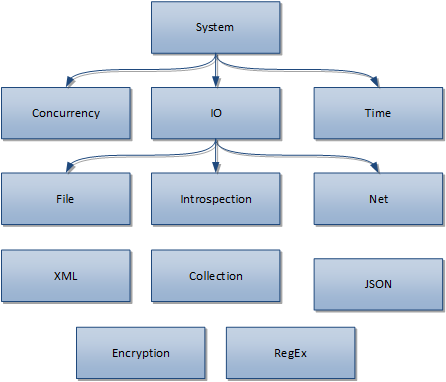
\includegraphics{../../images/classes.png}
\end{center}

Please refer to the online class library \htmladdnormallink{documentation}{http://www.objeck.org/docs/api/index.html} for additional information about bundles and classes.

\chapter{Examples}
\section{Prime Numbers}
Demonstrates basic language features such as arithmetic and logical
operations.
\begingroup
\fontsize{8pt}{9pt}\selectfont
\begin{verbatim}
class FindPrime {
  function : Main() ~ Nil {
    Run(1000000);
  }

  function : native : Run(topCandidate : Int)~ Nil {
    candidate : Int := 2;
    while(candidate <= topCandidate) {
      trialDivisor : Int := 2;
      prime : Int := 1;

      found : Bool := true;
      while(trialDivisor * trialDivisor <= candidate & found) {
        if(candidate % trialDivisor = 0) {
          prime := 0;
          found := false;
        }
        else {
          trialDivisor := trialDivisor + 1;
        };
      };

      if(found) {
        candidate->PrintLine();
      };
      candidate := candidate + 1;
    };
  }
}
\end{verbatim}
\endgroup
\section{Arrays}
Demonstrates the use of arrays.
\begingroup
\fontsize{8pt}{9pt}\selectfont
\begin{verbatim}
class Transpose {
  function : Main(args : String[]) ~ Nil {
    input := [
      [1, 1, 1, 1]
      [2, 4, 8, 16]
      [3, 9, 27, 81]
      [4, 16, 64, 256]
      [5, 25, 125, 625]
    ];
    dim := input->Size();

    output := Int->New[dim[0],dim[1]];
    for(i := 0; i < dim[0]; i+=1;) {
      for(j := 0; j < dim[1]; j+=1;) {
        output[i,j] := input[i,j];
      };
    };

    Print(output);
  }

  function : Print(matrix : Int[,]) ~ Nil {
    dim := matrix->Size();
    for(i := 0; i < dim[0]; i+=1;) {
      for(j := 0; j < dim[1]; j+=1;) {
        IO.Console->Print(matrix[i,j])->Print('\t');
      };
      '\n'->Print();
    };
  }
}
\end{verbatim}
\endgroup

\section{Simple HTTP client}
Demonstrates HTTP access.
\begingroup
\fontsize{8pt}{9pt}\selectfont
\begin{verbatim}
use Collection;

class HttpTest {
  client := HttpClient->New();
    # enable cookies
    client->CookiesEnabled(true);
    # request creates a cookie
    lines := client->Get("http://www.rexswain.com/cgi-bin/cookie.cgi?create");
    each(i : lines) {
      line := lines->Get(i)->As(String)->PrintLine();
    };
    # request sends back cookie
    lines := client->Get("http://www.rexswain.com/cgi-bin/cookie.cgi");
    each(i : lines) {
      line := lines->Get(i)->As(String)->PrintLine();
    };
  }
}
\end{verbatim}
\endgroup

\section{XML Parsing and Querying}
Demonstrates simple XML parsing.
\begingroup
\fontsize{8pt}{9pt}\selectfont
\begin{verbatim}
use System.IO;
use XML;

class Test {
  function : Main(args : String[]) ~ Nil {
    in := "";
    in += "<inventory title=\"OmniCorp Store #45x10^3\">";
    in += "<section name=\"health\">";
    in += "<item upc=\"123456789\" stock=\"12\">";
    in += "<name>Invisibility Cream</name>";
    in += "<price>14.50</price>";
    in += "<description>Makes you invisible</description>";
    in += "</item>";
    in += "<item upc=\"445322344\" stock=\"18\">";
    in += "<name>Levitation Salve</name>";
    in += "<price>23.99</price>";
    in += "<description>Levitate yourself for up to 3 hours per application</description>";
    in += "</item>";
    in += "</section>";
    in += "<section name=\"food\">";
    in += "<item upc=\"485672034\" stock=\"653\">";
    in += "<name>Blork and Freen Instameal</name>";
    in += "<price>4.95</price>";
    in += "<description>A tasty meal in a tablet; just add water</description>";
    in += "</item>";
    in += "<item upc=\"132957764\" stock=\"44\">";
    in += "<name>Grob winglets</name>";
    in += "<price>3.56</price>";
    in += "<description>Tender winglets of Grob. Just add water</description>";
    in += "</item>";
    in += "</section>";
    in += "</inventory>";
  
    parser := XmlParser->New(in);
    if(parser->Parse()) {
      # get first item
      results := parser->FindElements("/inventory/section[1]/item[1]");
      if(results <> Nil) {
        Console->Print("items: ")->PrintLine(results->Size());
      };
      # get all prices
      results := parser->FindElements("/inventory/section/item/price");
      if(results <> Nil) {
        each(i : results) {          
          element := results->Get(i)->As(XmlElement);
          element->GetContent()->PrintLine();
        };
      };
      # get names
      results := parser->FindElements("/inventory/section/item/name");
      if(results <> Nil) {
        Console->Print("names: ")->PrintLine(results->Size());
      };
    };
  }
}
\end{verbatim}
\endgroup

\section{Echo Server}
Demonstrates usage of server sockets and threads.
\begingroup
\fontsize{8pt}{9pt}\selectfont
\begin{verbatim}
use System.IO.Net;
use System.Concurrency;
 
bundle Default {
  class SocketServer {
    id : static : Int;
 
    function : Main(args : String[]) ~ Nil {
      server := TCPSocketServer->New(12321);
      if(server->Listen(5)) {
        while(true) {
          client := server->Accept();
          service := Service->New(id->ToString());
          service->Execute(client);
          id += 1;
        };
      };
      server->Close();
    }
  }
 
  class Service from Thread {
    New(name : String) {
      Parent(name);
    }
 
    method : public : Run(param : Base) ~ Nil {
      client := param->As(TCPSocket);
      line := client->ReadString();
      while(line->Size() > 0) {
        line->PrintLine();
        line := client->ReadString();
      };
    }
  }
}
\end{verbatim}
\endgroup

\chapter{Appendix A: Sample Debugging Session}
\section{Source for Example}
\begin{verbatim}
bundle Default {
  class Bar {
    v1 : Float;
    v2 : Int;

    New() {
      v1 := 2.31;
      v2 := 26;
    }
  }

  class Foo {
    bar : Bar;
    value : Int;

    New(v : Int) {
      value := v;
    }

    method : public : Get() ~ Int {
      return value;
    }

    method : public : SetBar() ~ Nil {
      bar := Bar->New();
    }
  }

  class Test {
    function : Main(args : System.String[]) ~ Nil {
      d : Float := 11.12;
      z := Int->New[5,6];
      z[2,3] := 27;

      f := Foo->New(24);
      f->SetBar();
      v := f->Get();
    }
  }
}
\end{verbatim}
The sample file is named \texttt{debug.obs}.

\section{Compiling the Source and Starting the Debugger}
\begin{verbatim}
obc -src test_src\debug.obs -dest a.obe -debug
obd -exe ..\..\compiler\a.obe -src ..\..\compiler\test_src

-------------------------------------
Objeck v1.0.0 - Interactive Debugger
-------------------------------------
loaded executable: file='../../compiler/a.obe'
source files: path='../../compiler/test_src/'
\end{verbatim}

\section{Setting a Breakpoint and Running the Program}
\begin{verbatim}
> b debug.obs:31
added break point: file='debug.obs:31'
> r
break: file='debug.obs:31', method='Test->Main(..)'
> l
  List
     26: 		}
     27: 	}
     28: 
     29: 	class Test {
     30: 		function : Main(args : System.String[]) ~ Nil {
=>   31: 			d : Float := 11.12;
     32: 			z := Int->New[5,6];	
     33: 			z[2,3] := 27;
     34: 
     35: 			f := Foo->New(24);
     36: 			f->SetBar();
> n
break: file='debug2.obs:32', method='Test->Main(..)'
\end{verbatim}

\section{Printing a Value}
\begin{verbatim}
> p d
print: type=Float, value=11.12
> b debug.obs:37
added break point: file='debug.obs:37'
> c
break: file='debug2.obs:37', method='Test->Main(..)'
> p z
print: type=Int[], value=2197556(0x218834), dimension=2, size=30
> p z[2,3]
print: type=Int[], value=27(0x1b)
>  p f->value
print: type=Int, value=24
> p f->bar
print: type=Bar, value=0x218864
> p f->bar->v1
print: type=Float, value=2.31
> q
> p f->bar->v1 * 3.5
print: type=Float, value=8.085
goodbye.
\end{verbatim}

\chapter{Appendix B: Compiler and VM Design}
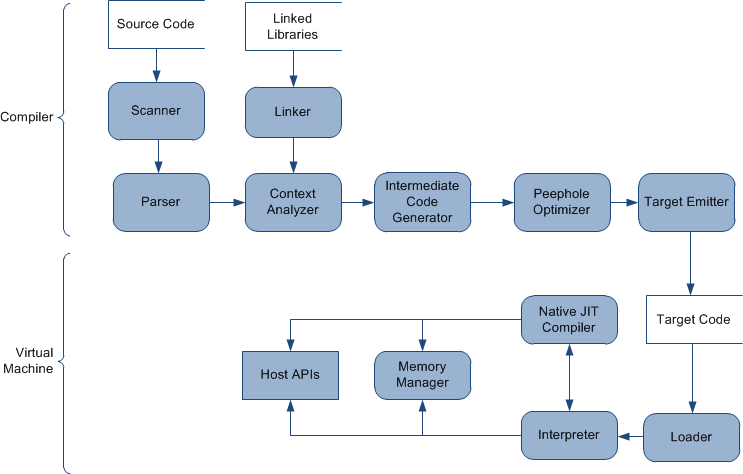
\includegraphics[scale=0.60]{../../images/compiler_data_flow.png}

The following section gives a brief overview of the major
architectural components the comprise the Objeck language compiler and
virtual machine.

\section{Compiler}
The language compiler is written in C++ and makes heavy use of the C++
STL for portability across platforms.  As mentioned in the
introduction, the compiler accepts source files and shared libraries
as inputs and produces either executables or shared libraries.  Note,
the compiler has two modes of operation: \texttt{User Mode} compiles
traditional end-user programs, while \texttt{System Mode} compiles
system libraries and processes special system language directives.

\subsection{Scanner and Parser}
The scanner component reads source files and parses the text into
tokens.  The scanner works in conjugation with the \emph{LL(k)} parser
by providing \emph{k} lookahead tokens for parsing.  Note, the scanner
can only scan system language directives while in \texttt{System
  Mode}.  The source parser is a recursive-decent parser that
generates an abstract parser tree, which is passed to the Contextual
Analyser for validation.

\subsection{Contextual Analyser}
The Contextual Analyzer is responsible for ensuring that a source
program is valid.  In addition, the context analyzer also creates
relationships between contextually resolved entities (i.e. methods
$\longleftrightarrow$ method calls).  The analyzer accepts an abstract
parser tree and shared libraries as input and produces a decorated
parse tree as output.  The decorated parse tree is then passed to the
Intermediate Code Generator for the production of VM instructions.

\subsection{Intermediate Code Generator and Optimzier}
The Intermediate Code Generator accpets a decorated parse and produces
a flat list of VM stack instructions.  These instruction lists are
then passed to the Optimizer for basic block optimizations (constant
folding, strength reduction, instruction simplification and method
inlining).

\subsection{Target Emitter}
Finally, the improved intermediate code is passed to code emitter
component, which writes it to a file.

\section{Virtual Machine}
The language VM is written in C/C++ and was designed to be highly
portable.  The VM makes heavy use of operating system specific APIs
(i.e. WIN32 and POSIX) but does so in an abstracted manner.  The JIT
compiler is targeted to produce machine code for the IA-32 and AMD64
hardware architectures.

\subsection{Loader}
The loader component allows the VM to read target code structures such
as classes, methods and VM instructions.  The loader create an
in-memory representation of this information, which is used by the VM
interpreter and JIT compiler.  In addition, the loader processes
command-line parameters that are passed into the VM prior to
execution.

\subsection{Interpreter}
The Interpreter executes stack based VM instructions (listed below)
and manages two primary stacks: the execution stack and call stack.
The execution stack is used to manage the data that is needed for VM
calculations.  The call stack is used to manage function/method calls
and the states between those calls.

\subsection{JIT Compiler}
The JIT compiler translates stack based VM instructions into processor
specific machine code (i.e. IA-32 and AMD64).  The JIT compiler is
evoked by the interpreter and methods are translated into machine code
and cached for subsequent calls.

\subsection{Memory Manager}
The Memory Manager component allows the runtime system to manage the
user allocation/deallocation of heap memory.  The memory mangers
implements a multi-thread ``mark and sweep'' algorithm.  The marking
stage of the process is multi-thread, such that, each root in scanned
in a separate thread.  The sweeping stage is done in a single thread
since runtime structures are modified.

\end{document}
